\chapter{Analyse}\label{ch:analyse}



\section{Motor}

\begin{figure}[ht!]
	\centering
	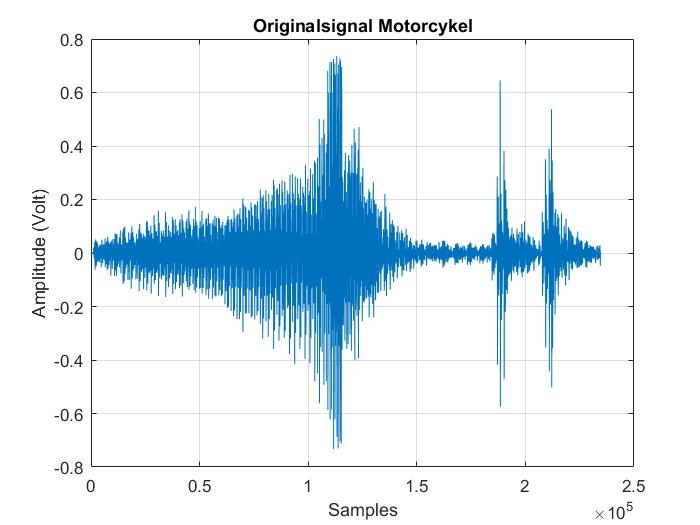
\includegraphics[width=180mm]{figures/Motor/original.jpg}
	\caption{DFT Det originale signal fra en Motor}
	\label{fig:Motor original}
\end{figure}

\begin{figure}[ht!]
	\centering
	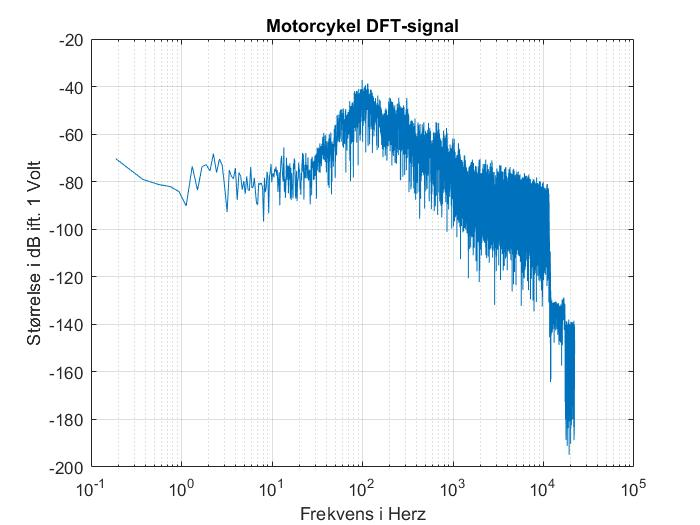
\includegraphics[width=180mm]{figures/Motor/DFT.jpg}
	\caption{DFT Analyse af et signal fra en Motor}
	\label{fig:Motor DFT}
\end{figure}

\begin{figure}[ht!]
	\centering
	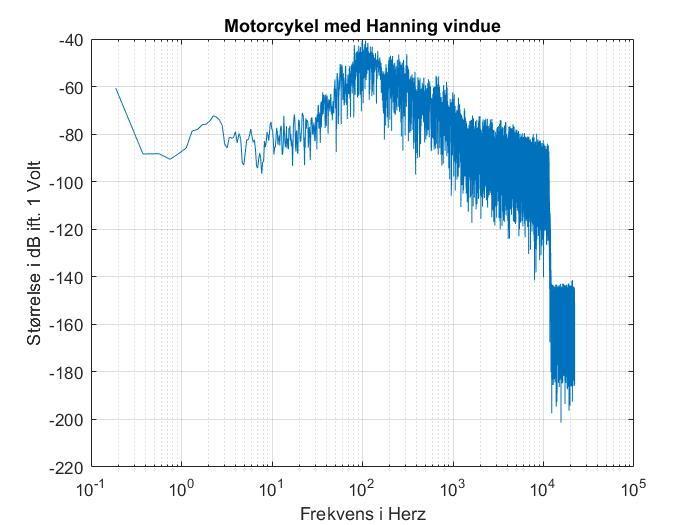
\includegraphics[width=180mm]{figures/Motor/hanning.jpg}
	\caption{DFT Analyse af et signal fra en Motor med et hanningvindue}
	\label{fig:Motor hanning}
\end{figure}

\begin{figure}[ht!]
	\centering
	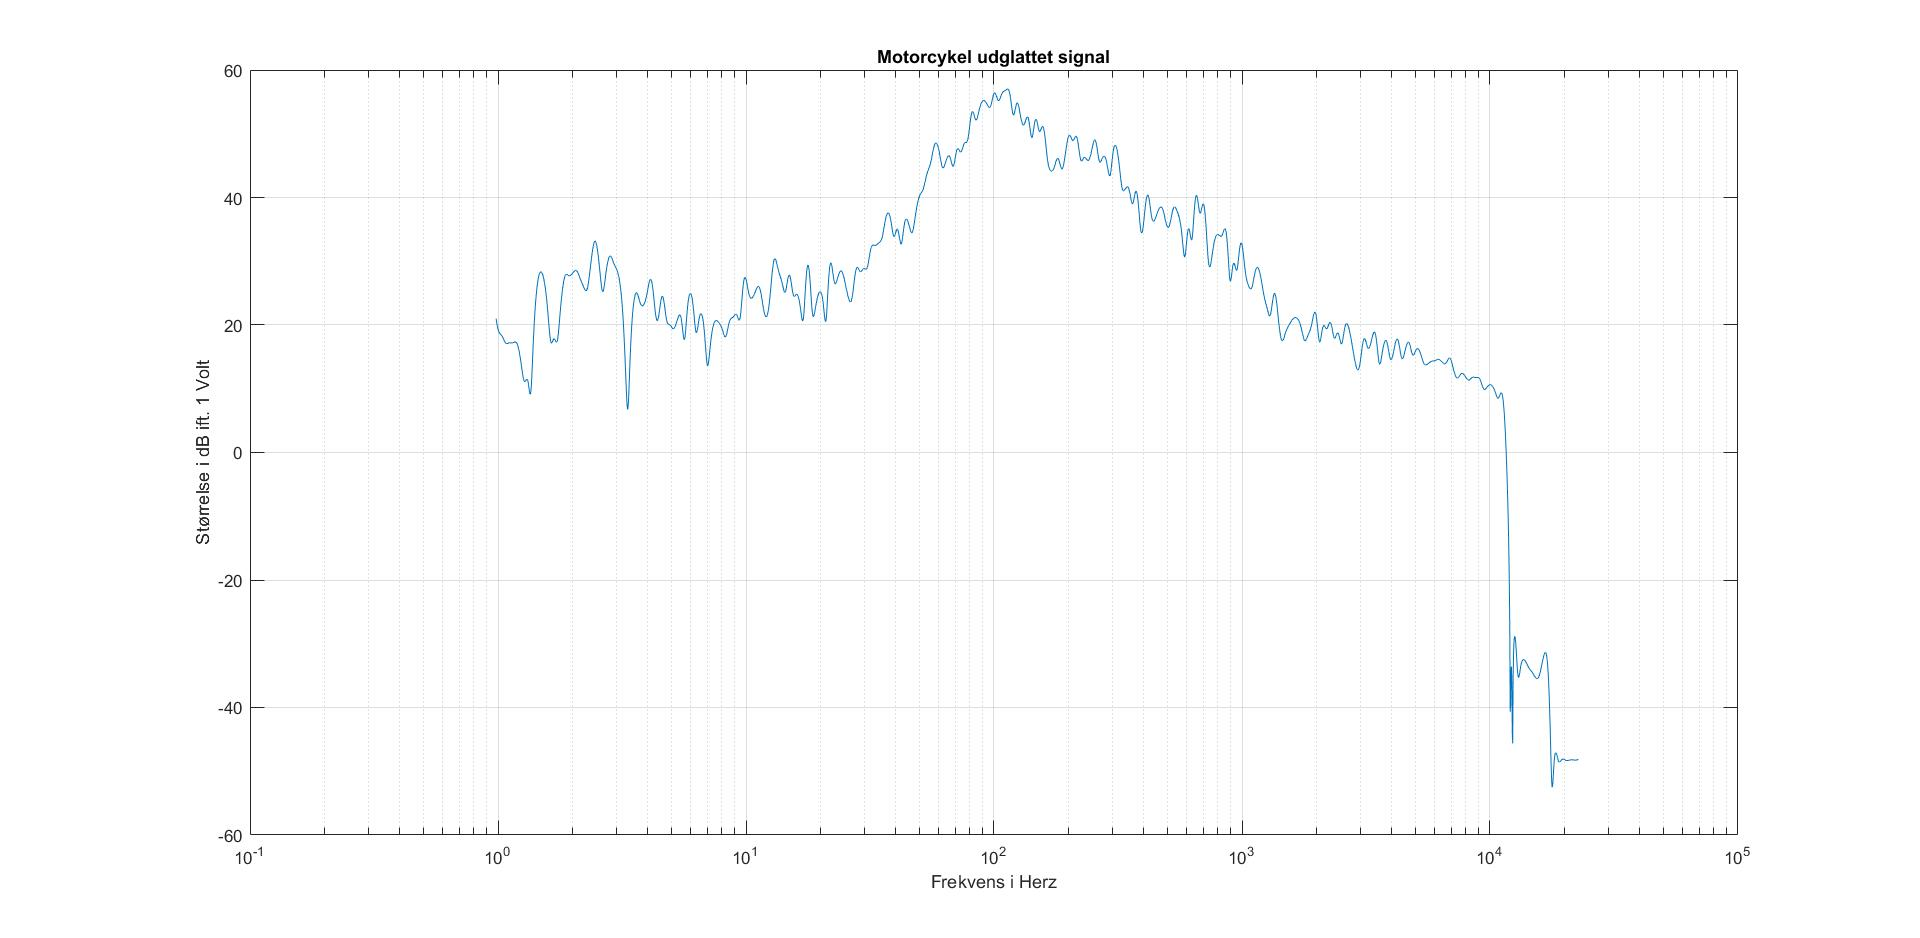
\includegraphics[width=180mm]{figures/Motor/udglattet.jpg}
	\caption{Det udglattede DFT signal fra en Motor}
	\label{fig:Motor udglattet}
\end{figure}

\section{Klaver}
\begin{figure}[ht!]
	\centering
	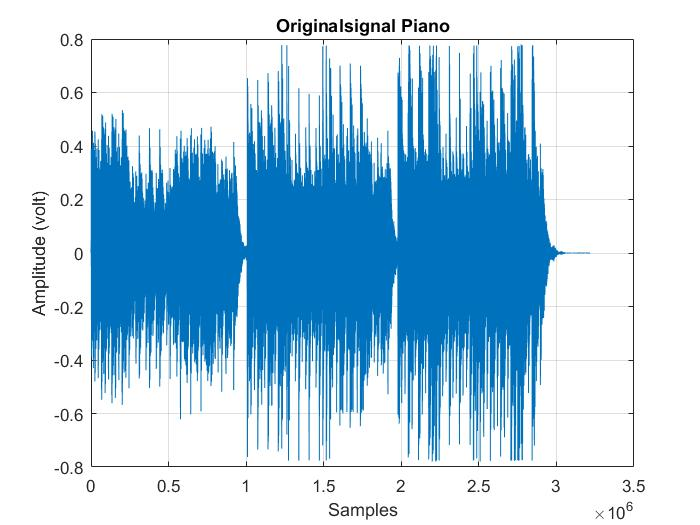
\includegraphics[width=180mm]{figures/Piano/original.jpg}
	\caption{DFT Det originale signal fra et klaver}
	\label{fig:Klaver original}
\end{figure}

\begin{figure}[ht!]
	\centering
	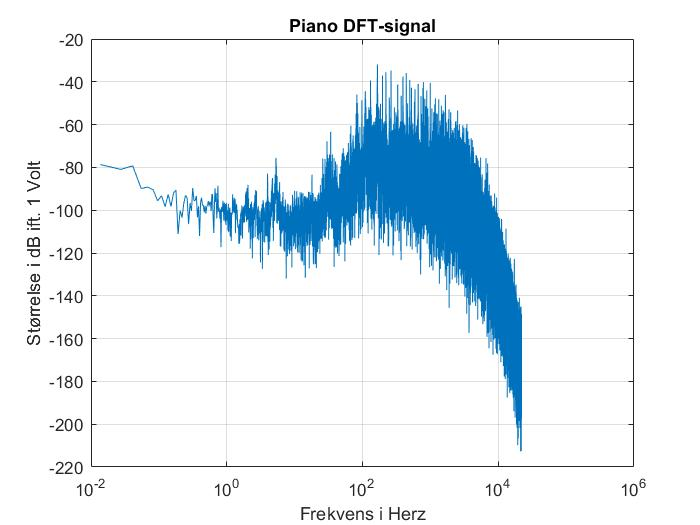
\includegraphics[width=180mm]{figures/Piano/DFT.jpg}
	\caption{DFT Analyse af et signal fra et Klaver}
	\label{fig:Klaver DFT}
\end{figure}

\begin{figure}[ht!]
	\centering
	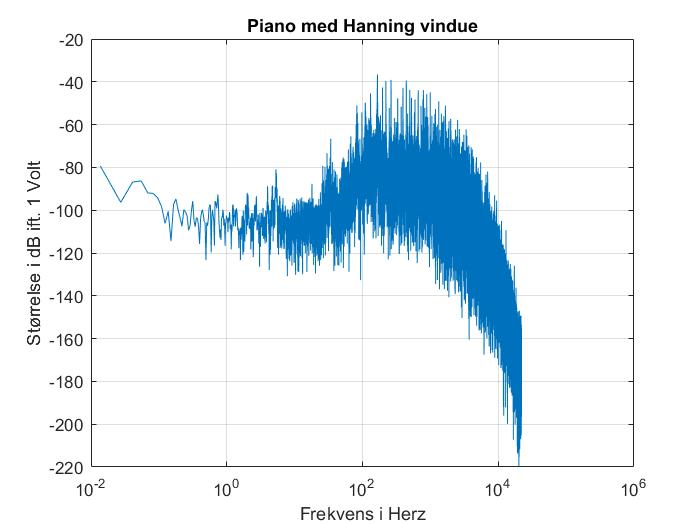
\includegraphics[width=180mm]{figures/Piano/hanning.jpg}
	\caption{DFT Analyse af et signal fra et klaver med et hanningvindue}
	\label{fig:Klaver hanning}
\end{figure}

\begin{figure}[ht!]
	\centering
	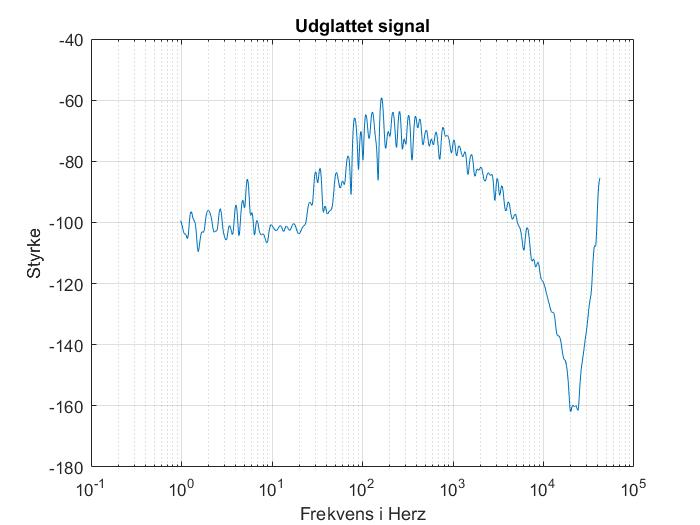
\includegraphics[width=180mm]{figures/Piano/udglattet.jpg}
	\caption{Det udglattede DFT signal fra et Klaver}
	\label{fig:Klaver udglattet}
\end{figure}


\section{Symfoni}



\section{Bass}



\section{Vinglas}


\section{Vindmølle}



\section{Musikbox}


\section{ECG-signal}

